%
\begin{isabellebody}%
\def\isabellecontext{Codegen}%
%
\isadelimtheory
\isanewline
%
\endisadelimtheory
%
\isatagtheory
%
\endisatagtheory
{\isafoldtheory}%
%
\isadelimtheory
%
\endisadelimtheory
%
\isadelimML
%
\endisadelimML
%
\isatagML
%
\endisatagML
{\isafoldML}%
%
\isadelimML
%
\endisadelimML
%
\isamarkupchapter{Code generation from Isabelle theories%
}
\isamarkuptrue%
%
\isamarkupsection{Introduction%
}
\isamarkuptrue%
%
\isamarkupsubsection{Motivation%
}
\isamarkuptrue%
%
\begin{isamarkuptext}%
Executing formal specifications as programs is a well-established
  topic in the theorem proving community.  With increasing
  application of theorem proving systems in the area of
  software development and verification, its relevance manifests
  for running test cases and rapid prototyping.  In logical
  calculi like constructive type theory,
  a notion of executability is implicit due to the nature
  of the calculus.  In contrast, specifications in Isabelle
  can be highly non-executable.  In order to bridge
  the gap between logic and executable specifications,
  an explicit non-trivial transformation has to be applied:
  code generation.

  This tutorial introduces a generic code generator for the
  Isabelle system \cite{isa-tutorial}.
  Generic in the sense that the
  \qn{target language} for which code shall ultimately be
  generated is not fixed but may be an arbitrary state-of-the-art
  functional programming language (currently, the implementation
  supports SML \cite{SML}, OCaml \cite{OCaml} and Haskell
  \cite{haskell-revised-report}).
  We aim to provide a
  versatile environment
  suitable for software development and verification,
  structuring the process
  of code generation into a small set of orthogonal principles
  while achieving a big coverage of application areas
  with maximum flexibility.

  Conceptually the code generator framework is part
  of Isabelle's \isa{Pure} meta logic; the object logic
  \isa{HOL} which is an extension of \isa{Pure}
  already comes with a reasonable framework setup and thus provides
  a good working horse for raising code-generation-driven
  applications.  So, we assume some familiarity and experience
  with the ingredients of the \isa{HOL} \emph{Main} theory
  (see also \cite{isa-tutorial}).%
\end{isamarkuptext}%
\isamarkuptrue%
%
\isamarkupsubsection{Overview%
}
\isamarkuptrue%
%
\begin{isamarkuptext}%
The code generator aims to be usable with no further ado
  in most cases while allowing for detailed customization.
  This manifests in the structure of this tutorial:
  we start with a generic example \secref{sec:example}
  and introduce code generation concepts \secref{sec:concept}.
  Section
  \secref{sec:basics} explains how to use the framework naively,
  presuming a reasonable default setup.  Then, section
  \secref{sec:advanced} deals with advanced topics,
  introducing further aspects of the code generator framework
  in a motivation-driven manner.  Last, section \secref{sec:ml}
  introduces the framework's internal programming interfaces.

  \begin{warn}
    Ultimately, the code generator which this tutorial deals with
    is supposed to replace the already established code generator
    by Stefan Berghofer \cite{Berghofer-Nipkow:2002}.
    So, for the moment, there are two distinct code generators
    in Isabelle.
    Also note that while the framework itself is
    object-logic independent, only \isa{HOL} provides a reasonable
    framework setup.    
  \end{warn}%
\end{isamarkuptext}%
\isamarkuptrue%
%
\isamarkupsection{An example: a simple theory of search trees \label{sec:example}%
}
\isamarkuptrue%
%
\begin{isamarkuptext}%
When writing executable specifications using \isa{HOL},
  it is convenient to use
  three existing packages: the datatype package for defining
  datatypes, the function package for (recursive) functions,
  and the class package for overloaded definitions.

  We develope a small theory of search trees; trees are represented
  as a datatype with key type \isa{{\isacharprime}a} and value type \isa{{\isacharprime}b}:%
\end{isamarkuptext}%
\isamarkuptrue%
\isacommand{datatype}\isamarkupfalse%
\ {\isacharparenleft}{\isacharprime}a{\isacharcomma}\ {\isacharprime}b{\isacharparenright}\ searchtree\ {\isacharequal}\ Leaf\ {\isachardoublequoteopen}{\isacharprime}a{\isasymColon}linorder{\isachardoublequoteclose}\ {\isacharprime}b\isanewline
\ \ {\isacharbar}\ Branch\ {\isachardoublequoteopen}{\isacharparenleft}{\isacharprime}a{\isacharcomma}\ {\isacharprime}b{\isacharparenright}\ searchtree{\isachardoublequoteclose}\ {\isachardoublequoteopen}{\isacharprime}a{\isachardoublequoteclose}\ {\isachardoublequoteopen}{\isacharparenleft}{\isacharprime}a{\isacharcomma}\ {\isacharprime}b{\isacharparenright}\ searchtree{\isachardoublequoteclose}%
\begin{isamarkuptext}%
\noindent Note that we have constrained the type of keys
  to the class of total orders, \isa{linorder}.

  We define \isa{find} and \isa{update} functions:%
\end{isamarkuptext}%
\isamarkuptrue%
\isacommand{fun}\isamarkupfalse%
\isanewline
\ \ find\ {\isacharcolon}{\isacharcolon}\ {\isachardoublequoteopen}{\isacharparenleft}{\isacharprime}a{\isasymColon}linorder{\isacharcomma}\ {\isacharprime}b{\isacharparenright}\ searchtree\ {\isasymRightarrow}\ {\isacharprime}a\ {\isasymRightarrow}\ {\isacharprime}b\ option{\isachardoublequoteclose}\ \isakeyword{where}\isanewline
\ \ {\isachardoublequoteopen}find\ {\isacharparenleft}Leaf\ key\ val{\isacharparenright}\ it\ {\isacharequal}\ {\isacharparenleft}if\ it\ {\isacharequal}\ key\ then\ Some\ val\ else\ None{\isacharparenright}{\isachardoublequoteclose}\isanewline
\ \ {\isacharbar}\ {\isachardoublequoteopen}find\ {\isacharparenleft}Branch\ t{\isadigit{1}}\ key\ t{\isadigit{2}}{\isacharparenright}\ it\ {\isacharequal}\ {\isacharparenleft}if\ it\ {\isasymle}\ key\ then\ find\ t{\isadigit{1}}\ it\ else\ find\ t{\isadigit{2}}\ it{\isacharparenright}{\isachardoublequoteclose}\isanewline
\isanewline
\isacommand{fun}\isamarkupfalse%
\isanewline
\ \ update\ {\isacharcolon}{\isacharcolon}\ {\isachardoublequoteopen}{\isacharprime}a{\isasymColon}linorder\ {\isasymtimes}\ {\isacharprime}b\ {\isasymRightarrow}\ {\isacharparenleft}{\isacharprime}a{\isacharcomma}\ {\isacharprime}b{\isacharparenright}\ searchtree\ {\isasymRightarrow}\ {\isacharparenleft}{\isacharprime}a{\isacharcomma}\ {\isacharprime}b{\isacharparenright}\ searchtree{\isachardoublequoteclose}\ \isakeyword{where}\isanewline
\ \ {\isachardoublequoteopen}update\ {\isacharparenleft}it{\isacharcomma}\ entry{\isacharparenright}\ {\isacharparenleft}Leaf\ key\ val{\isacharparenright}\ {\isacharequal}\ {\isacharparenleft}\isanewline
\ \ \ \ if\ it\ {\isacharequal}\ key\ then\ Leaf\ key\ entry\isanewline
\ \ \ \ \ \ else\ if\ it\ {\isasymle}\ key\isanewline
\ \ \ \ \ \ then\ Branch\ {\isacharparenleft}Leaf\ it\ entry{\isacharparenright}\ it\ {\isacharparenleft}Leaf\ key\ val{\isacharparenright}\isanewline
\ \ \ \ \ \ else\ Branch\ {\isacharparenleft}Leaf\ key\ val{\isacharparenright}\ it\ {\isacharparenleft}Leaf\ it\ entry{\isacharparenright}\isanewline
\ \ \ {\isacharparenright}{\isachardoublequoteclose}\isanewline
\ \ {\isacharbar}\ {\isachardoublequoteopen}update\ {\isacharparenleft}it{\isacharcomma}\ entry{\isacharparenright}\ {\isacharparenleft}Branch\ t{\isadigit{1}}\ key\ t{\isadigit{2}}{\isacharparenright}\ {\isacharequal}\ {\isacharparenleft}\isanewline
\ \ \ \ if\ it\ {\isasymle}\ key\isanewline
\ \ \ \ \ \ then\ {\isacharparenleft}Branch\ {\isacharparenleft}update\ {\isacharparenleft}it{\isacharcomma}\ entry{\isacharparenright}\ t{\isadigit{1}}{\isacharparenright}\ key\ t{\isadigit{2}}{\isacharparenright}\isanewline
\ \ \ \ \ \ else\ {\isacharparenleft}Branch\ t{\isadigit{1}}\ key\ {\isacharparenleft}update\ {\isacharparenleft}it{\isacharcomma}\ entry{\isacharparenright}\ t{\isadigit{2}}{\isacharparenright}{\isacharparenright}\isanewline
\ \ \ {\isacharparenright}{\isachardoublequoteclose}%
\begin{isamarkuptext}%
\noindent For testing purpose, we define a small example
  using natural numbers \isa{nat} (which are a \isa{linorder})
  as keys and list of nats as values:%
\end{isamarkuptext}%
\isamarkuptrue%
\isacommand{definition}\isamarkupfalse%
\isanewline
\ \ example\ {\isacharcolon}{\isacharcolon}\ {\isachardoublequoteopen}{\isacharparenleft}nat{\isacharcomma}\ nat\ list{\isacharparenright}\ searchtree{\isachardoublequoteclose}\isanewline
\isakeyword{where}\isanewline
\ \ {\isachardoublequoteopen}example\ {\isacharequal}\ update\ {\isacharparenleft}Suc\ {\isacharparenleft}Suc\ {\isacharparenleft}Suc\ {\isacharparenleft}Suc\ {\isadigit{0}}{\isacharparenright}{\isacharparenright}{\isacharparenright}{\isacharcomma}\ {\isacharbrackleft}Suc\ {\isacharparenleft}Suc\ {\isadigit{0}}{\isacharparenright}{\isacharcomma}\ Suc\ {\isacharparenleft}Suc\ {\isadigit{0}}{\isacharparenright}{\isacharbrackright}{\isacharparenright}\ {\isacharparenleft}update\ {\isacharparenleft}Suc\ {\isacharparenleft}Suc\ {\isacharparenleft}Suc\ {\isadigit{0}}{\isacharparenright}{\isacharparenright}{\isacharcomma}\ {\isacharbrackleft}Suc\ {\isacharparenleft}Suc\ {\isacharparenleft}Suc\ {\isadigit{0}}{\isacharparenright}{\isacharparenright}{\isacharbrackright}{\isacharparenright}\isanewline
\ \ \ \ {\isacharparenleft}update\ {\isacharparenleft}Suc\ {\isacharparenleft}Suc\ {\isadigit{0}}{\isacharparenright}{\isacharcomma}\ {\isacharbrackleft}Suc\ {\isacharparenleft}Suc\ {\isadigit{0}}{\isacharparenright}{\isacharbrackright}{\isacharparenright}\ {\isacharparenleft}Leaf\ {\isacharparenleft}Suc\ {\isadigit{0}}{\isacharparenright}\ {\isacharbrackleft}{\isacharbrackright}{\isacharparenright}{\isacharparenright}{\isacharparenright}{\isachardoublequoteclose}%
\begin{isamarkuptext}%
\noindent Then we generate code%
\end{isamarkuptext}%
\isamarkuptrue%
\isacommand{export{\isacharunderscore}code}\isamarkupfalse%
\ example\ \isakeyword{in}\ SML\ \isakeyword{file}\ {\isachardoublequoteopen}examples{\isacharslash}tree{\isachardot}ML{\isachardoublequoteclose}%
\begin{isamarkuptext}%
\noindent which looks like:
  \lstsml{Thy/examples/tree.ML}%
\end{isamarkuptext}%
\isamarkuptrue%
%
\isamarkupsection{Code generation concepts and process \label{sec:concept}%
}
\isamarkuptrue%
%
\begin{isamarkuptext}%
\begin{figure}[h]
  \centering
  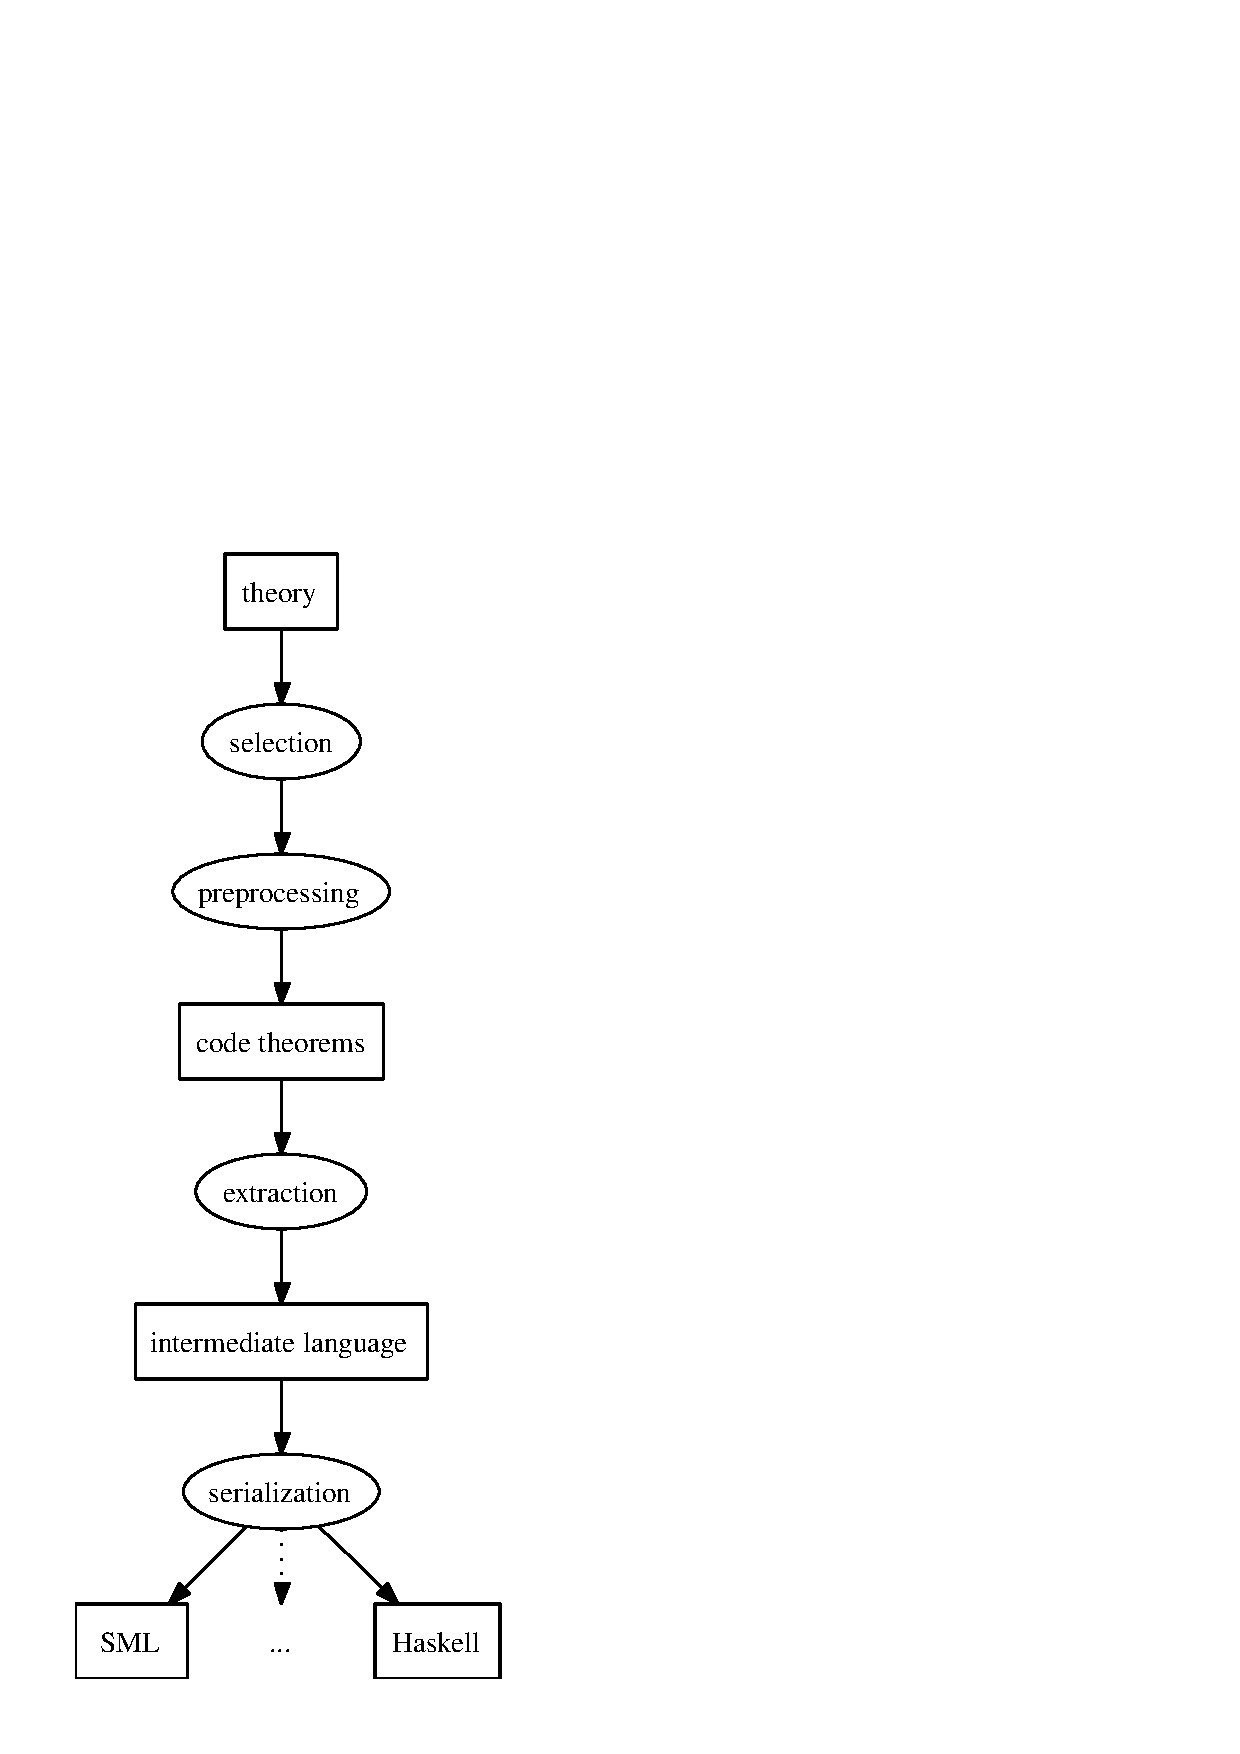
\includegraphics[width=0.7\textwidth]{codegen_process}
  \caption{code generator -- processing overview}
  \label{fig:process}
  \end{figure}

  The code generator employs a notion of executability
  for three foundational executable ingredients known
  from functional programming:
  \emph{defining equations}, \emph{datatypes}, and
  \emph{type classes}. A defining equation as a first approximation
  is a theorem of the form \isa{f\ t\isactrlisub {\isadigit{1}}\ t\isactrlisub {\isadigit{2}}\ {\isasymdots}\ t\isactrlisub n\ {\isasymequiv}\ t}
  (an equation headed by a constant \isa{f} with arguments
  \isa{t\isactrlisub {\isadigit{1}}\ t\isactrlisub {\isadigit{2}}\ {\isasymdots}\ t\isactrlisub n} and right hand side \isa{t}).
  Code generation aims to turn defining equations
  into a functional program by running through
  a process (see figure \ref{fig:process}):

  \begin{itemize}

    \item Out of the vast collection of theorems proven in a
      \qn{theory}, a reasonable subset modeling
      defining equations is \qn{selected}.

    \item On those selected theorems, certain
      transformations are carried out
      (\qn{preprocessing}).  Their purpose is to turn theorems
      representing non- or badly executable
      specifications into equivalent but executable counterparts.
      The result is a structured collection of \qn{code theorems}.

    \item These \qn{code theorems} then are \qn{translated}
      into an Haskell-like intermediate
      language.

    \item Finally, out of the intermediate language the final
      code in the desired \qn{target language} is \qn{serialized}.

  \end{itemize}

  From these steps, only the two last are carried out
  outside the logic; by keeping this layer as
  thin as possible, the amount of code to trust is
  kept to a minimum.%
\end{isamarkuptext}%
\isamarkuptrue%
%
\isamarkupsection{Basics \label{sec:basics}%
}
\isamarkuptrue%
%
\isamarkupsubsection{Invoking the code generator%
}
\isamarkuptrue%
%
\begin{isamarkuptext}%
Thanks to a reasonable setup of the \isa{HOL} theories, in
  most cases code generation proceeds without further ado:%
\end{isamarkuptext}%
\isamarkuptrue%
\isacommand{fun}\isamarkupfalse%
\isanewline
\ \ fac\ {\isacharcolon}{\isacharcolon}\ {\isachardoublequoteopen}nat\ {\isasymRightarrow}\ nat{\isachardoublequoteclose}\ \isakeyword{where}\isanewline
\ \ \ \ {\isachardoublequoteopen}fac\ {\isadigit{0}}\ {\isacharequal}\ {\isadigit{1}}{\isachardoublequoteclose}\isanewline
\ \ {\isacharbar}\ {\isachardoublequoteopen}fac\ {\isacharparenleft}Suc\ n{\isacharparenright}\ {\isacharequal}\ Suc\ n\ {\isacharasterisk}\ fac\ n{\isachardoublequoteclose}%
\begin{isamarkuptext}%
\noindent This executable specification is now turned to SML code:%
\end{isamarkuptext}%
\isamarkuptrue%
\isacommand{export{\isacharunderscore}code}\isamarkupfalse%
\ fac\ \isakeyword{in}\ SML\ \isakeyword{file}\ {\isachardoublequoteopen}examples{\isacharslash}fac{\isachardot}ML{\isachardoublequoteclose}%
\begin{isamarkuptext}%
\noindent  The \isa{{\isasymEXPORTCODE}} command takes a space-separated list of
  constants together with \qn{serialization directives}
  These start with a \qn{target language}
  identifier, followed by a file specification
  where to write the generated code to.

  Internally, the defining equations for all selected
  constants are taken, including any transitively required
  constants, datatypes and classes, resulting in the following
  code:

  \lstsml{Thy/examples/fac.ML}

  The code generator will complain when a required
  ingredient does not provide a executable counterpart,
  e.g.~generating code
  for constants not yielding
  a defining equation (e.g.~the Hilbert choice
  operation \isa{SOME}):%
\end{isamarkuptext}%
\isamarkuptrue%
%
\isadelimML
%
\endisadelimML
%
\isatagML
%
\endisatagML
{\isafoldML}%
%
\isadelimML
%
\endisadelimML
\isacommand{definition}\isamarkupfalse%
\isanewline
\ \ pick{\isacharunderscore}some\ {\isacharcolon}{\isacharcolon}\ {\isachardoublequoteopen}{\isacharprime}a\ list\ {\isasymRightarrow}\ {\isacharprime}a{\isachardoublequoteclose}\ \isakeyword{where}\isanewline
\ \ {\isachardoublequoteopen}pick{\isacharunderscore}some\ xs\ {\isacharequal}\ {\isacharparenleft}SOME\ x{\isachardot}\ x\ {\isasymin}\ set\ xs{\isacharparenright}{\isachardoublequoteclose}%
\isadelimML
%
\endisadelimML
%
\isatagML
%
\endisatagML
{\isafoldML}%
%
\isadelimML
%
\endisadelimML
\isacommand{export{\isacharunderscore}code}\isamarkupfalse%
\ pick{\isacharunderscore}some\ \isakeyword{in}\ SML\ \isakeyword{file}\ {\isachardoublequoteopen}examples{\isacharslash}fail{\isacharunderscore}const{\isachardot}ML{\isachardoublequoteclose}%
\begin{isamarkuptext}%
\noindent will fail.%
\end{isamarkuptext}%
\isamarkuptrue%
%
\isamarkupsubsection{Theorem selection%
}
\isamarkuptrue%
%
\begin{isamarkuptext}%
The list of all defining equations in a theory may be inspected
  using the \isa{{\isasymPRINTCODESETUP}} command:%
\end{isamarkuptext}%
\isamarkuptrue%
\isacommand{print{\isacharunderscore}codesetup}\isamarkupfalse%
%
\begin{isamarkuptext}%
\noindent which displays a table of constant with corresponding
  defining equations (the additional stuff displayed
  shall not bother us for the moment).

  The typical \isa{HOL} tools are already set up in a way that
  function definitions introduced by \isa{{\isasymDEFINITION}},
  \isa{{\isasymFUN}},
  \isa{{\isasymFUNCTION}}, \isa{{\isasymPRIMREC}},
  \isa{{\isasymRECDEF}} are implicitly propagated
  to this defining equation table. Specific theorems may be
  selected using an attribute: \emph{code func}. As example,
  a weight selector function:%
\end{isamarkuptext}%
\isamarkuptrue%
\isacommand{consts}\isamarkupfalse%
\isanewline
\ \ pick\ {\isacharcolon}{\isacharcolon}\ {\isachardoublequoteopen}{\isacharparenleft}nat\ {\isasymtimes}\ {\isacharprime}a{\isacharparenright}\ list\ {\isasymRightarrow}\ nat\ {\isasymRightarrow}\ {\isacharprime}a{\isachardoublequoteclose}\isanewline
\isanewline
\isacommand{primrec}\isamarkupfalse%
\isanewline
\ \ {\isachardoublequoteopen}pick\ {\isacharparenleft}x{\isacharhash}xs{\isacharparenright}\ n\ {\isacharequal}\ {\isacharparenleft}let\ {\isacharparenleft}k{\isacharcomma}\ v{\isacharparenright}\ {\isacharequal}\ x\ in\isanewline
\ \ \ \ if\ n\ {\isacharless}\ k\ then\ v\ else\ pick\ xs\ {\isacharparenleft}n\ {\isacharminus}\ k{\isacharparenright}{\isacharparenright}{\isachardoublequoteclose}%
\begin{isamarkuptext}%
\noindent We want to eliminate the explicit destruction
  of \isa{x} to \isa{{\isacharparenleft}k{\isacharcomma}\ v{\isacharparenright}}:%
\end{isamarkuptext}%
\isamarkuptrue%
\isacommand{lemma}\isamarkupfalse%
\ {\isacharbrackleft}code\ func{\isacharbrackright}{\isacharcolon}\isanewline
\ \ {\isachardoublequoteopen}pick\ {\isacharparenleft}{\isacharparenleft}k{\isacharcomma}\ v{\isacharparenright}{\isacharhash}xs{\isacharparenright}\ n\ {\isacharequal}\ {\isacharparenleft}if\ n\ {\isacharless}\ k\ then\ v\ else\ pick\ xs\ {\isacharparenleft}n\ {\isacharminus}\ k{\isacharparenright}{\isacharparenright}{\isachardoublequoteclose}\isanewline
%
\isadelimproof
\ \ %
\endisadelimproof
%
\isatagproof
\isacommand{by}\isamarkupfalse%
\ simp%
\endisatagproof
{\isafoldproof}%
%
\isadelimproof
\isanewline
%
\endisadelimproof
\isanewline
\isacommand{export{\isacharunderscore}code}\isamarkupfalse%
\ pick\ \ \isakeyword{in}\ SML\ \isakeyword{file}\ {\isachardoublequoteopen}examples{\isacharslash}pick{\isadigit{1}}{\isachardot}ML{\isachardoublequoteclose}%
\begin{isamarkuptext}%
\noindent This theorem now is used for generating code:

  \lstsml{Thy/examples/pick1.ML}

  \noindent It might be convenient to remove the pointless original
  equation, using the \emph{func del} attribute:%
\end{isamarkuptext}%
\isamarkuptrue%
\isacommand{lemmas}\isamarkupfalse%
\ {\isacharbrackleft}code\ func\ del{\isacharbrackright}\ {\isacharequal}\ pick{\isachardot}simps\ \isanewline
\isanewline
\isacommand{export{\isacharunderscore}code}\isamarkupfalse%
\ pick\ \ \isakeyword{in}\ SML\ \isakeyword{file}\ {\isachardoublequoteopen}examples{\isacharslash}pick{\isadigit{2}}{\isachardot}ML{\isachardoublequoteclose}%
\begin{isamarkuptext}%
\lstsml{Thy/examples/pick2.ML}

  \noindent Syntactic redundancies are implicitly dropped. For example,
  using a modified version of the \isa{fac} function
  as defining equation, the then redundant (since
  syntactically subsumed) original defining equations
  are dropped, resulting in a warning:%
\end{isamarkuptext}%
\isamarkuptrue%
\isacommand{lemma}\isamarkupfalse%
\ {\isacharbrackleft}code\ func{\isacharbrackright}{\isacharcolon}\isanewline
\ \ {\isachardoublequoteopen}fac\ n\ {\isacharequal}\ {\isacharparenleft}case\ n\ of\ {\isadigit{0}}\ {\isasymRightarrow}\ {\isadigit{1}}\ {\isacharbar}\ Suc\ m\ {\isasymRightarrow}\ n\ {\isacharasterisk}\ fac\ m{\isacharparenright}{\isachardoublequoteclose}\isanewline
%
\isadelimproof
\ \ %
\endisadelimproof
%
\isatagproof
\isacommand{by}\isamarkupfalse%
\ {\isacharparenleft}cases\ n{\isacharparenright}\ simp{\isacharunderscore}all%
\endisatagproof
{\isafoldproof}%
%
\isadelimproof
\isanewline
%
\endisadelimproof
\isanewline
\isacommand{export{\isacharunderscore}code}\isamarkupfalse%
\ fac\ \isakeyword{in}\ SML\ \isakeyword{file}\ {\isachardoublequoteopen}examples{\isacharslash}fac{\isacharunderscore}case{\isachardot}ML{\isachardoublequoteclose}%
\begin{isamarkuptext}%
\lstsml{Thy/examples/fac_case.ML}

  \begin{warn}
    The attributes \emph{code} and \emph{code del}
    associated with the existing code generator also apply to
    the new one: \emph{code} implies \emph{code func},
    and \emph{code del} implies \emph{code func del}.
  \end{warn}%
\end{isamarkuptext}%
\isamarkuptrue%
%
\isamarkupsubsection{Type classes%
}
\isamarkuptrue%
%
\begin{isamarkuptext}%
Type classes enter the game via the Isar class package.
  For a short introduction how to use it, see \cite{isabelle-classes};
  here we just illustrate its impact on code generation.

  In a target language, type classes may be represented
  natively (as in the case of Haskell).  For languages
  like SML, they are implemented using \emph{dictionaries}.
  Our following example specifies a class \qt{null},
  assigning to each of its inhabitants a \qt{null} value:%
\end{isamarkuptext}%
\isamarkuptrue%
\isacommand{class}\isamarkupfalse%
\ null\ {\isacharequal}\ type\ {\isacharplus}\isanewline
\ \ \isakeyword{fixes}\ null\ {\isacharcolon}{\isacharcolon}\ {\isacharprime}a\isanewline
\isanewline
\isacommand{fun}\isamarkupfalse%
\isanewline
\ \ head\ {\isacharcolon}{\isacharcolon}\ {\isachardoublequoteopen}{\isacharprime}a{\isasymColon}null\ list\ {\isasymRightarrow}\ {\isacharprime}a{\isachardoublequoteclose}\isanewline
\isakeyword{where}\isanewline
\ \ {\isachardoublequoteopen}head\ {\isacharbrackleft}{\isacharbrackright}\ {\isacharequal}\ null{\isachardoublequoteclose}\isanewline
\ \ {\isacharbar}\ {\isachardoublequoteopen}head\ {\isacharparenleft}x{\isacharhash}xs{\isacharparenright}\ {\isacharequal}\ x{\isachardoublequoteclose}%
\begin{isamarkuptext}%
\noindent  We provide some instances for our \isa{null}:%
\end{isamarkuptext}%
\isamarkuptrue%
\isacommand{instantiation}\isamarkupfalse%
\ option\ \isakeyword{and}\ list\ {\isacharcolon}{\isacharcolon}\ {\isacharparenleft}type{\isacharparenright}\ null\isanewline
\isakeyword{begin}\isanewline
\isanewline
\isacommand{definition}\isamarkupfalse%
\isanewline
\ \ {\isachardoublequoteopen}null\ {\isacharequal}\ None{\isachardoublequoteclose}\isanewline
\isanewline
\isacommand{definition}\isamarkupfalse%
\isanewline
\ \ {\isachardoublequoteopen}null\ {\isacharequal}\ {\isacharbrackleft}{\isacharbrackright}{\isachardoublequoteclose}\isanewline
\isanewline
\isacommand{instance}\isamarkupfalse%
%
\isadelimproof
\ %
\endisadelimproof
%
\isatagproof
\isacommand{{\isachardot}{\isachardot}}\isamarkupfalse%
%
\endisatagproof
{\isafoldproof}%
%
\isadelimproof
%
\endisadelimproof
\isanewline
\isanewline
\isacommand{end}\isamarkupfalse%
%
\begin{isamarkuptext}%
\noindent Constructing a dummy example:%
\end{isamarkuptext}%
\isamarkuptrue%
\isacommand{definition}\isamarkupfalse%
\isanewline
\ \ {\isachardoublequoteopen}dummy\ {\isacharequal}\ head\ {\isacharbrackleft}Some\ {\isacharparenleft}Suc\ {\isadigit{0}}{\isacharparenright}{\isacharcomma}\ None{\isacharbrackright}{\isachardoublequoteclose}%
\begin{isamarkuptext}%
Type classes offer a suitable occasion to introduce
  the Haskell serializer.  Its usage is almost the same
  as SML, but, in accordance with conventions
  some Haskell systems enforce, each module ends
  up in a single file. The module hierarchy is reflected in
  the file system, with root directory given as file specification.%
\end{isamarkuptext}%
\isamarkuptrue%
\isacommand{export{\isacharunderscore}code}\isamarkupfalse%
\ dummy\ \isakeyword{in}\ Haskell\ \isakeyword{file}\ {\isachardoublequoteopen}examples{\isacharslash}{\isachardoublequoteclose}%
\begin{isamarkuptext}%
\lsthaskell{Thy/examples/Codegen.hs}
  \noindent (we have left out all other modules).

  \medskip

  The whole code in SML with explicit dictionary passing:%
\end{isamarkuptext}%
\isamarkuptrue%
\isacommand{export{\isacharunderscore}code}\isamarkupfalse%
\ dummy\ \isakeyword{in}\ SML\ \isakeyword{file}\ {\isachardoublequoteopen}examples{\isacharslash}class{\isachardot}ML{\isachardoublequoteclose}%
\begin{isamarkuptext}%
\lstsml{Thy/examples/class.ML}

  \medskip

  \noindent or in OCaml:%
\end{isamarkuptext}%
\isamarkuptrue%
\isacommand{export{\isacharunderscore}code}\isamarkupfalse%
\ dummy\ \isakeyword{in}\ OCaml\ \isakeyword{file}\ {\isachardoublequoteopen}examples{\isacharslash}class{\isachardot}ocaml{\isachardoublequoteclose}%
\begin{isamarkuptext}%
\lstsml{Thy/examples/class.ocaml}

  \medskip The explicit association of constants
  to classes can be inspected using the \isa{{\isasymPRINTCLASSES}}
  command.%
\end{isamarkuptext}%
\isamarkuptrue%
%
\isamarkupsection{Recipes and advanced topics \label{sec:advanced}%
}
\isamarkuptrue%
%
\begin{isamarkuptext}%
In this tutorial, we do not attempt to give an exhaustive
  description of the code generator framework; instead,
  we cast a light on advanced topics by introducing
  them together with practically motivated examples.  Concerning
  further reading, see

  \begin{itemize}

  \item the Isabelle/Isar Reference Manual \cite{isabelle-isar-ref}
    for exhaustive syntax diagrams.
  \item or \cite{Haftmann-Nipkow:2007:codegen} which deals with foundational issues
    of the code generator framework.

  \end{itemize}%
\end{isamarkuptext}%
\isamarkuptrue%
%
\isamarkupsubsection{Library theories \label{sec:library}%
}
\isamarkuptrue%
%
\begin{isamarkuptext}%
The \isa{HOL} \isa{Main} theory already provides a code
  generator setup
  which should be suitable for most applications. Common extensions
  and modifications are available by certain theories of the \isa{HOL}
  library; beside being useful in applications, they may serve
  as a tutorial for customizing the code generator setup.

  \begin{description}

    \item[\isa{Code{\isacharunderscore}Integer}] represents \isa{HOL} integers by big
       integer literals in target languages.
    \item[\isa{Code{\isacharunderscore}Char}] represents \isa{HOL} characters by 
       character literals in target languages.
    \item[\isa{Code{\isacharunderscore}Char{\isacharunderscore}chr}] like \isa{Code{\isacharunderscore}Char},
       but also offers treatment of character codes; includes
       \isa{Code{\isacharunderscore}Integer}.
    \item[\isa{Efficient{\isacharunderscore}Nat}] \label{eff_nat} implements natural numbers by integers,
       which in general will result in higher efficency; pattern
       matching with \isa{{\isadigit{0}}} / \isa{Suc}
       is eliminated;  includes \isa{Code{\isacharunderscore}Integer}.
    \item[\isa{Code{\isacharunderscore}Index}] provides an additional datatype
       \isa{index} which is mapped to target-language built-in integers.
       Useful for code setups which involve e.g. indexing of
       target-language arrays.
    \item[\isa{Code{\isacharunderscore}Message}] provides an additional datatype
       \isa{message{\isacharunderscore}string} which is isomorphic to strings;
       \isa{message{\isacharunderscore}string}s are mapped to target-language strings.
       Useful for code setups which involve e.g. printing (error) messages.

  \end{description}

  \begin{warn}
    When importing any of these theories, they should form the last
    items in an import list.  Since these theories adapt the
    code generator setup in a non-conservative fashion,
    strange effects may occur otherwise.
  \end{warn}%
\end{isamarkuptext}%
\isamarkuptrue%
%
\isamarkupsubsection{Preprocessing%
}
\isamarkuptrue%
%
\begin{isamarkuptext}%
Before selected function theorems are turned into abstract
  code, a chain of definitional transformation steps is carried
  out: \emph{preprocessing}. There are three possibilities
  to customize preprocessing: \emph{inline theorems},
  \emph{inline procedures} and \emph{generic preprocessors}.

  \emph{Inline theorems} are rewriting rules applied to each
  defining equation.  Due to the interpretation of theorems
  of defining equations, rewrites are applied to the right
  hand side and the arguments of the left hand side of an
  equation, but never to the constant heading the left hand side.
  Inline theorems may be declared an undeclared using the
  \emph{code inline} or \emph{code inline del} attribute respectively.
  Some common applications:%
\end{isamarkuptext}%
\isamarkuptrue%
%
\begin{itemize}
%
\begin{isamarkuptext}%
\item replacing non-executable constructs by executable ones:%
\end{isamarkuptext}%
\isamarkuptrue%
\ \ \isacommand{lemma}\isamarkupfalse%
\ {\isacharbrackleft}code\ inline{\isacharbrackright}{\isacharcolon}\isanewline
\ \ \ \ {\isachardoublequoteopen}x\ {\isasymin}\ set\ xs\ {\isasymlongleftrightarrow}\ x\ mem\ xs{\isachardoublequoteclose}%
\isadelimproof
\ %
\endisadelimproof
%
\isatagproof
\isacommand{by}\isamarkupfalse%
\ {\isacharparenleft}induct\ xs{\isacharparenright}\ simp{\isacharunderscore}all%
\endisatagproof
{\isafoldproof}%
%
\isadelimproof
%
\endisadelimproof
%
\begin{isamarkuptext}%
\item eliminating superfluous constants:%
\end{isamarkuptext}%
\isamarkuptrue%
\ \ \isacommand{lemma}\isamarkupfalse%
\ {\isacharbrackleft}code\ inline{\isacharbrackright}{\isacharcolon}\isanewline
\ \ \ \ {\isachardoublequoteopen}{\isadigit{1}}\ {\isacharequal}\ Suc\ {\isadigit{0}}{\isachardoublequoteclose}%
\isadelimproof
\ %
\endisadelimproof
%
\isatagproof
\isacommand{by}\isamarkupfalse%
\ simp%
\endisatagproof
{\isafoldproof}%
%
\isadelimproof
%
\endisadelimproof
%
\begin{isamarkuptext}%
\item replacing executable but inconvenient constructs:%
\end{isamarkuptext}%
\isamarkuptrue%
\ \ \isacommand{lemma}\isamarkupfalse%
\ {\isacharbrackleft}code\ inline{\isacharbrackright}{\isacharcolon}\isanewline
\ \ \ \ {\isachardoublequoteopen}xs\ {\isacharequal}\ {\isacharbrackleft}{\isacharbrackright}\ {\isasymlongleftrightarrow}\ List{\isachardot}null\ xs{\isachardoublequoteclose}%
\isadelimproof
\ %
\endisadelimproof
%
\isatagproof
\isacommand{by}\isamarkupfalse%
\ {\isacharparenleft}induct\ xs{\isacharparenright}\ simp{\isacharunderscore}all%
\endisatagproof
{\isafoldproof}%
%
\isadelimproof
%
\endisadelimproof
%
\end{itemize}
%
\begin{isamarkuptext}%
\noindent The current set of inline theorems may be inspected using
  the \isa{{\isasymPRINTCODESETUP}} command.

  \emph{Inline procedures} are a generalized version of inline
  theorems written in ML -- rewrite rules are generated dependent
  on the function theorems for a certain function.  One
  application is the implicit expanding of \isa{nat} numerals
  to \isa{{\isadigit{0}}} / \isa{Suc} representation.  See further
  \secref{sec:ml}

  \emph{Generic preprocessors} provide a most general interface,
  transforming a list of function theorems to another
  list of function theorems, provided that neither the heading
  constant nor its type change.  The \isa{{\isadigit{0}}} / \isa{Suc}
  pattern elimination implemented in
  theory \isa{EfficientNat} (\secref{eff_nat}) uses this
  interface.

  \begin{warn}
    The order in which single preprocessing steps are carried
    out currently is not specified; in particular, preprocessing
    is \emph{no} fix point process.  Keep this in mind when
    setting up the preprocessor.

    Further, the attribute \emph{code unfold}
    associated with the existing code generator also applies to
    the new one: \emph{code unfold} implies \emph{code inline}.
  \end{warn}%
\end{isamarkuptext}%
\isamarkuptrue%
%
\isamarkupsubsection{Concerning operational equality%
}
\isamarkuptrue%
%
\begin{isamarkuptext}%
Surely you have already noticed how equality is treated
  by the code generator:%
\end{isamarkuptext}%
\isamarkuptrue%
\isacommand{fun}\isamarkupfalse%
\isanewline
\ \ collect{\isacharunderscore}duplicates\ {\isacharcolon}{\isacharcolon}\ {\isachardoublequoteopen}{\isacharprime}a\ list\ {\isasymRightarrow}\ {\isacharprime}a\ list\ {\isasymRightarrow}\ {\isacharprime}a\ list\ {\isasymRightarrow}\ {\isacharprime}a\ list{\isachardoublequoteclose}\ \isakeyword{where}\isanewline
\ \ \ \ {\isachardoublequoteopen}collect{\isacharunderscore}duplicates\ xs\ ys\ {\isacharbrackleft}{\isacharbrackright}\ {\isacharequal}\ xs{\isachardoublequoteclose}\isanewline
\ \ {\isacharbar}\ {\isachardoublequoteopen}collect{\isacharunderscore}duplicates\ xs\ ys\ {\isacharparenleft}z{\isacharhash}zs{\isacharparenright}\ {\isacharequal}\ {\isacharparenleft}if\ z\ {\isasymin}\ set\ xs\isanewline
\ \ \ \ \ \ then\ if\ z\ {\isasymin}\ set\ ys\isanewline
\ \ \ \ \ \ \ \ then\ collect{\isacharunderscore}duplicates\ xs\ ys\ zs\isanewline
\ \ \ \ \ \ \ \ else\ collect{\isacharunderscore}duplicates\ xs\ {\isacharparenleft}z{\isacharhash}ys{\isacharparenright}\ zs\isanewline
\ \ \ \ \ \ else\ collect{\isacharunderscore}duplicates\ {\isacharparenleft}z{\isacharhash}xs{\isacharparenright}\ {\isacharparenleft}z{\isacharhash}ys{\isacharparenright}\ zs{\isacharparenright}{\isachardoublequoteclose}%
\begin{isamarkuptext}%
The membership test during preprocessing is rewritten,
  resulting in \isa{op\ mem}, which itself
  performs an explicit equality check.%
\end{isamarkuptext}%
\isamarkuptrue%
\isacommand{export{\isacharunderscore}code}\isamarkupfalse%
\ collect{\isacharunderscore}duplicates\ \isakeyword{in}\ SML\ \isakeyword{file}\ {\isachardoublequoteopen}examples{\isacharslash}collect{\isacharunderscore}duplicates{\isachardot}ML{\isachardoublequoteclose}%
\begin{isamarkuptext}%
\lstsml{Thy/examples/collect_duplicates.ML}%
\end{isamarkuptext}%
\isamarkuptrue%
%
\begin{isamarkuptext}%
Obviously, polymorphic equality is implemented the Haskell
  way using a type class.  How is this achieved?  By an
  almost trivial definition in the HOL setup:%
\end{isamarkuptext}%
\isamarkuptrue%
%
\isadelimML
%
\endisadelimML
%
\isatagML
%
\endisatagML
{\isafoldML}%
%
\isadelimML
%
\endisadelimML
\isacommand{class}\isamarkupfalse%
\ eq\ {\isacharparenleft}\isakeyword{attach}\ {\isachardoublequoteopen}op\ {\isacharequal}{\isachardoublequoteclose}{\isacharparenright}\ {\isacharequal}\ type%
\begin{isamarkuptext}%
This merely introduces a class \isa{eq} with corresponding
  operation \isa{op\ {\isacharequal}};
  the preprocessing framework does the rest.
  For datatypes, instances of \isa{eq} are implicitly derived
  when possible.

  Though this \isa{eq} class is designed to get rarely in
  the way, a subtlety
  enters the stage when definitions of overloaded constants
  are dependent on operational equality.  For example, let
  us define a lexicographic ordering on tuples:%
\end{isamarkuptext}%
\isamarkuptrue%
%
\isadelimML
%
\endisadelimML
%
\isatagML
%
\endisatagML
{\isafoldML}%
%
\isadelimML
%
\endisadelimML
\isacommand{instance}\isamarkupfalse%
\ {\isacharasterisk}\ {\isacharcolon}{\isacharcolon}\ {\isacharparenleft}ord{\isacharcomma}\ ord{\isacharparenright}\ ord\isanewline
\ \ less{\isacharunderscore}prod{\isacharunderscore}def{\isacharcolon}\isanewline
\ \ \ \ {\isachardoublequoteopen}p{\isadigit{1}}\ {\isacharless}\ p{\isadigit{2}}\ {\isasymequiv}\ let\ {\isacharparenleft}x{\isadigit{1}}\ {\isasymColon}\ {\isacharprime}a{\isasymColon}ord{\isacharcomma}\ y{\isadigit{1}}\ {\isasymColon}\ {\isacharprime}b{\isasymColon}ord{\isacharparenright}\ {\isacharequal}\ p{\isadigit{1}}{\isacharsemicolon}\ {\isacharparenleft}x{\isadigit{2}}{\isacharcomma}\ y{\isadigit{2}}{\isacharparenright}\ {\isacharequal}\ p{\isadigit{2}}\ in\isanewline
\ \ \ \ x{\isadigit{1}}\ {\isacharless}\ x{\isadigit{2}}\ {\isasymor}\ {\isacharparenleft}x{\isadigit{1}}\ {\isacharequal}\ x{\isadigit{2}}\ {\isasymand}\ y{\isadigit{1}}\ {\isacharless}\ y{\isadigit{2}}{\isacharparenright}{\isachardoublequoteclose}\isanewline
\ \ less{\isacharunderscore}eq{\isacharunderscore}prod{\isacharunderscore}def{\isacharcolon}\isanewline
\ \ \ \ {\isachardoublequoteopen}p{\isadigit{1}}\ {\isasymle}\ p{\isadigit{2}}\ {\isasymequiv}\ let\ {\isacharparenleft}x{\isadigit{1}}\ {\isasymColon}\ {\isacharprime}a{\isasymColon}ord{\isacharcomma}\ y{\isadigit{1}}\ {\isasymColon}\ {\isacharprime}b{\isasymColon}ord{\isacharparenright}\ {\isacharequal}\ p{\isadigit{1}}{\isacharsemicolon}\ {\isacharparenleft}x{\isadigit{2}}{\isacharcomma}\ y{\isadigit{2}}{\isacharparenright}\ {\isacharequal}\ p{\isadigit{2}}\ in\isanewline
\ \ \ \ x{\isadigit{1}}\ {\isacharless}\ x{\isadigit{2}}\ {\isasymor}\ {\isacharparenleft}x{\isadigit{1}}\ {\isacharequal}\ x{\isadigit{2}}\ {\isasymand}\ y{\isadigit{1}}\ {\isasymle}\ y{\isadigit{2}}{\isacharparenright}{\isachardoublequoteclose}%
\isadelimproof
\ %
\endisadelimproof
%
\isatagproof
\isacommand{{\isachardot}{\isachardot}}\isamarkupfalse%
%
\endisatagproof
{\isafoldproof}%
%
\isadelimproof
%
\endisadelimproof
\isanewline
\isanewline
\isacommand{lemmas}\isamarkupfalse%
\ {\isacharbrackleft}code\ func\ del{\isacharbrackright}\ {\isacharequal}\ less{\isacharunderscore}prod{\isacharunderscore}def\ less{\isacharunderscore}eq{\isacharunderscore}prod{\isacharunderscore}def\isanewline
\isanewline
\isacommand{lemma}\isamarkupfalse%
\ ord{\isacharunderscore}prod\ {\isacharbrackleft}code\ func{\isacharbrackright}{\isacharcolon}\isanewline
\ \ {\isachardoublequoteopen}{\isacharparenleft}x{\isadigit{1}}\ {\isasymColon}\ {\isacharprime}a{\isasymColon}ord{\isacharcomma}\ y{\isadigit{1}}\ {\isasymColon}\ {\isacharprime}b{\isasymColon}ord{\isacharparenright}\ {\isacharless}\ {\isacharparenleft}x{\isadigit{2}}{\isacharcomma}\ y{\isadigit{2}}{\isacharparenright}\ {\isasymlongleftrightarrow}\ x{\isadigit{1}}\ {\isacharless}\ x{\isadigit{2}}\ {\isasymor}\ {\isacharparenleft}x{\isadigit{1}}\ {\isacharequal}\ x{\isadigit{2}}\ {\isasymand}\ y{\isadigit{1}}\ {\isacharless}\ y{\isadigit{2}}{\isacharparenright}{\isachardoublequoteclose}\isanewline
\ \ {\isachardoublequoteopen}{\isacharparenleft}x{\isadigit{1}}\ {\isasymColon}\ {\isacharprime}a{\isasymColon}ord{\isacharcomma}\ y{\isadigit{1}}\ {\isasymColon}\ {\isacharprime}b{\isasymColon}ord{\isacharparenright}\ {\isasymle}\ {\isacharparenleft}x{\isadigit{2}}{\isacharcomma}\ y{\isadigit{2}}{\isacharparenright}\ {\isasymlongleftrightarrow}\ x{\isadigit{1}}\ {\isacharless}\ x{\isadigit{2}}\ {\isasymor}\ {\isacharparenleft}x{\isadigit{1}}\ {\isacharequal}\ x{\isadigit{2}}\ {\isasymand}\ y{\isadigit{1}}\ {\isasymle}\ y{\isadigit{2}}{\isacharparenright}{\isachardoublequoteclose}\isanewline
%
\isadelimproof
\ \ %
\endisadelimproof
%
\isatagproof
\isacommand{unfolding}\isamarkupfalse%
\ less{\isacharunderscore}prod{\isacharunderscore}def\ less{\isacharunderscore}eq{\isacharunderscore}prod{\isacharunderscore}def\ \isacommand{by}\isamarkupfalse%
\ simp{\isacharunderscore}all%
\endisatagproof
{\isafoldproof}%
%
\isadelimproof
%
\endisadelimproof
%
\begin{isamarkuptext}%
Then code generation will fail.  Why?  The definition
  of \isa{op\ {\isasymle}} depends on equality on both arguments,
  which are polymorphic and impose an additional \isa{eq}
  class constraint, thus violating the type discipline
  for class operations.

  The solution is to add \isa{eq} explicitly to the first sort arguments in the
  code theorems:%
\end{isamarkuptext}%
\isamarkuptrue%
\isacommand{lemma}\isamarkupfalse%
\ ord{\isacharunderscore}prod{\isacharunderscore}code\ {\isacharbrackleft}code\ func{\isacharbrackright}{\isacharcolon}\isanewline
\ \ {\isachardoublequoteopen}{\isacharparenleft}x{\isadigit{1}}\ {\isasymColon}\ {\isacharprime}a{\isasymColon}{\isacharbraceleft}ord{\isacharcomma}\ eq{\isacharbraceright}{\isacharcomma}\ y{\isadigit{1}}\ {\isasymColon}\ {\isacharprime}b{\isasymColon}ord{\isacharparenright}\ {\isacharless}\ {\isacharparenleft}x{\isadigit{2}}{\isacharcomma}\ y{\isadigit{2}}{\isacharparenright}\ {\isasymlongleftrightarrow}\isanewline
\ \ \ \ x{\isadigit{1}}\ {\isacharless}\ x{\isadigit{2}}\ {\isasymor}\ {\isacharparenleft}x{\isadigit{1}}\ {\isacharequal}\ x{\isadigit{2}}\ {\isasymand}\ y{\isadigit{1}}\ {\isacharless}\ y{\isadigit{2}}{\isacharparenright}{\isachardoublequoteclose}\isanewline
\ \ {\isachardoublequoteopen}{\isacharparenleft}x{\isadigit{1}}\ {\isasymColon}\ {\isacharprime}a{\isasymColon}{\isacharbraceleft}ord{\isacharcomma}\ eq{\isacharbraceright}{\isacharcomma}\ y{\isadigit{1}}\ {\isasymColon}\ {\isacharprime}b{\isasymColon}ord{\isacharparenright}\ {\isasymle}\ {\isacharparenleft}x{\isadigit{2}}{\isacharcomma}\ y{\isadigit{2}}{\isacharparenright}\ {\isasymlongleftrightarrow}\isanewline
\ \ \ \ x{\isadigit{1}}\ {\isacharless}\ x{\isadigit{2}}\ {\isasymor}\ {\isacharparenleft}x{\isadigit{1}}\ {\isacharequal}\ x{\isadigit{2}}\ {\isasymand}\ y{\isadigit{1}}\ {\isasymle}\ y{\isadigit{2}}{\isacharparenright}{\isachardoublequoteclose}\isanewline
%
\isadelimproof
\ \ %
\endisadelimproof
%
\isatagproof
\isacommand{unfolding}\isamarkupfalse%
\ ord{\isacharunderscore}prod\ \isacommand{by}\isamarkupfalse%
\ rule{\isacharplus}%
\endisatagproof
{\isafoldproof}%
%
\isadelimproof
%
\endisadelimproof
%
\begin{isamarkuptext}%
\noindent Then code generation succeeds:%
\end{isamarkuptext}%
\isamarkuptrue%
\isacommand{export{\isacharunderscore}code}\isamarkupfalse%
\ {\isachardoublequoteopen}op\ {\isasymle}\ {\isasymColon}\ {\isacharprime}a{\isasymColon}{\isacharbraceleft}eq{\isacharcomma}\ ord{\isacharbraceright}\ {\isasymtimes}\ {\isacharprime}b{\isasymColon}ord\ {\isasymRightarrow}\ {\isacharprime}a\ {\isasymtimes}\ {\isacharprime}b\ {\isasymRightarrow}\ bool{\isachardoublequoteclose}\isanewline
\ \ \isakeyword{in}\ SML\ \isakeyword{file}\ {\isachardoublequoteopen}examples{\isacharslash}lexicographic{\isachardot}ML{\isachardoublequoteclose}%
\begin{isamarkuptext}%
\lstsml{Thy/examples/lexicographic.ML}%
\end{isamarkuptext}%
\isamarkuptrue%
%
\begin{isamarkuptext}%
In general, code theorems for overloaded constants may have more
  restrictive sort constraints than the underlying instance relation
  between class and type constructor as long as the whole system of
  constraints is coregular; code theorems violating coregularity
  are rejected immediately.  Consequently, it might be necessary
  to delete disturbing theorems in the code theorem table,
  as we have done here with the original definitions \isa{less{\isacharunderscore}prod{\isacharunderscore}def}
  and \isa{less{\isacharunderscore}eq{\isacharunderscore}prod{\isacharunderscore}def}.

  In some cases, the automatically derived defining equations
  for equality on a particular type may not be appropriate.
  As example, watch the following datatype representing
  monomorphic parametric types (where type constructors
  are referred to by natural numbers):%
\end{isamarkuptext}%
\isamarkuptrue%
\isacommand{datatype}\isamarkupfalse%
\ monotype\ {\isacharequal}\ Mono\ nat\ {\isachardoublequoteopen}monotype\ list{\isachardoublequoteclose}%
\isadelimproof
%
\endisadelimproof
%
\isatagproof
%
\endisatagproof
{\isafoldproof}%
%
\isadelimproof
%
\endisadelimproof
%
\begin{isamarkuptext}%
Then code generation for SML would fail with a message
  that the generated code conains illegal mutual dependencies:
  the theorem \isa{Mono\ tyco{\isadigit{1}}\ typargs{\isadigit{1}}\ {\isacharequal}\ Mono\ tyco{\isadigit{2}}\ typargs{\isadigit{2}}\ {\isasymequiv}\ tyco{\isadigit{1}}\ {\isacharequal}\ tyco{\isadigit{2}}\ {\isasymand}\ typargs{\isadigit{1}}\ {\isacharequal}\ typargs{\isadigit{2}}} already requires the
  instance \isa{monotype\ {\isasymColon}\ eq}, which itself requires
  \isa{Mono\ tyco{\isadigit{1}}\ typargs{\isadigit{1}}\ {\isacharequal}\ Mono\ tyco{\isadigit{2}}\ typargs{\isadigit{2}}\ {\isasymequiv}\ tyco{\isadigit{1}}\ {\isacharequal}\ tyco{\isadigit{2}}\ {\isasymand}\ typargs{\isadigit{1}}\ {\isacharequal}\ typargs{\isadigit{2}}};  Haskell has no problem with mutually
  recursive \isa{instance} and \isa{function} definitions,
  but the SML serializer does not support this.

  In such cases, you have to provide you own equality equations
  involving auxiliary constants.  In our case,
  \isa{list{\isacharunderscore}all{\isadigit{2}}} can do the job:%
\end{isamarkuptext}%
\isamarkuptrue%
\isacommand{lemma}\isamarkupfalse%
\ monotype{\isacharunderscore}eq{\isacharunderscore}list{\isacharunderscore}all{\isadigit{2}}\ {\isacharbrackleft}code\ func{\isacharbrackright}{\isacharcolon}\isanewline
\ \ {\isachardoublequoteopen}Mono\ tyco{\isadigit{1}}\ typargs{\isadigit{1}}\ {\isacharequal}\ Mono\ tyco{\isadigit{2}}\ typargs{\isadigit{2}}\ {\isasymlongleftrightarrow}\isanewline
\ \ \ \ \ tyco{\isadigit{1}}\ {\isacharequal}\ tyco{\isadigit{2}}\ {\isasymand}\ list{\isacharunderscore}all{\isadigit{2}}\ {\isacharparenleft}op\ {\isacharequal}{\isacharparenright}\ typargs{\isadigit{1}}\ typargs{\isadigit{2}}{\isachardoublequoteclose}\isanewline
%
\isadelimproof
\ \ %
\endisadelimproof
%
\isatagproof
\isacommand{by}\isamarkupfalse%
\ {\isacharparenleft}simp\ add{\isacharcolon}\ list{\isacharunderscore}all{\isadigit{2}}{\isacharunderscore}eq\ {\isacharbrackleft}symmetric{\isacharbrackright}{\isacharparenright}%
\endisatagproof
{\isafoldproof}%
%
\isadelimproof
%
\endisadelimproof
%
\begin{isamarkuptext}%
does not depend on instance \isa{monotype\ {\isasymColon}\ eq}:%
\end{isamarkuptext}%
\isamarkuptrue%
\isacommand{export{\isacharunderscore}code}\isamarkupfalse%
\ {\isachardoublequoteopen}op\ {\isacharequal}\ {\isacharcolon}{\isacharcolon}\ monotype\ {\isasymRightarrow}\ monotype\ {\isasymRightarrow}\ bool{\isachardoublequoteclose}\isanewline
\ \ \isakeyword{in}\ SML\ \isakeyword{file}\ {\isachardoublequoteopen}examples{\isacharslash}monotype{\isachardot}ML{\isachardoublequoteclose}%
\begin{isamarkuptext}%
\lstsml{Thy/examples/monotype.ML}%
\end{isamarkuptext}%
\isamarkuptrue%
%
\isamarkupsubsection{Programs as sets of theorems%
}
\isamarkuptrue%
%
\begin{isamarkuptext}%
As told in \secref{sec:concept}, code generation is based
  on a structured collection of code theorems.
  For explorative purpose, this collection
  may be inspected using the \isa{{\isasymCODETHMS}} command:%
\end{isamarkuptext}%
\isamarkuptrue%
\isacommand{code{\isacharunderscore}thms}\isamarkupfalse%
\ {\isachardoublequoteopen}op\ mod\ {\isacharcolon}{\isacharcolon}\ nat\ {\isasymRightarrow}\ nat\ {\isasymRightarrow}\ nat{\isachardoublequoteclose}%
\begin{isamarkuptext}%
\noindent prints a table with \emph{all} defining equations
  for \isa{op\ mod}, including
  \emph{all} defining equations those equations depend
  on recursivly.  \isa{{\isasymCODETHMS}} provides a convenient
  mechanism to inspect the impact of a preprocessor setup
  on defining equations.
  
  Similarly, the \isa{{\isasymCODEDEPS}} command shows a graph
  visualizing dependencies between defining equations.%
\end{isamarkuptext}%
\isamarkuptrue%
%
\isamarkupsubsection{Constructor sets for datatypes%
}
\isamarkuptrue%
%
\begin{isamarkuptext}%
Conceptually, any datatype is spanned by a set of
  \emph{constructors} of type \isa{{\isasymtau}\ {\isacharequal}\ {\isasymdots}\ {\isasymRightarrow}\ {\isasymkappa}\ {\isasymalpha}\isactrlisub {\isadigit{1}}\ {\isasymdots}\ {\isasymalpha}\isactrlisub n}
  where \isa{{\isacharbraceleft}{\isasymalpha}\isactrlisub {\isadigit{1}}{\isacharcomma}\ {\isasymdots}{\isacharcomma}\ {\isasymalpha}\isactrlisub n{\isacharbraceright}} is excactly the set of \emph{all}
  type variables in \isa{{\isasymtau}}.  The HOL datatype package
  by default registers any new datatype in the table
  of datatypes, which may be inspected using
  the \isa{{\isasymPRINTCODESETUP}} command.

  In some cases, it may be convenient to alter or
  extend this table;  as an example, we show
  how to implement finite sets by lists
  using the conversion \isa{{\isachardoublequote}set\ {\isasymColon}\ {\isacharprime}a\ list\ {\isasymRightarrow}\ {\isacharprime}a\ set{\isachardoublequote}}
  as constructor:%
\end{isamarkuptext}%
\isamarkuptrue%
\ %
\isadelimML
%
\endisadelimML
%
\isatagML
%
\endisatagML
{\isafoldML}%
%
\isadelimML
%
\endisadelimML
\isanewline
\isacommand{code{\isacharunderscore}datatype}\isamarkupfalse%
\ set\isanewline
\isanewline
\isacommand{lemma}\isamarkupfalse%
\ {\isacharbrackleft}code\ func{\isacharbrackright}{\isacharcolon}\ {\isachardoublequoteopen}{\isacharbraceleft}{\isacharbraceright}\ {\isacharequal}\ set\ {\isacharbrackleft}{\isacharbrackright}{\isachardoublequoteclose}%
\isadelimproof
\ %
\endisadelimproof
%
\isatagproof
\isacommand{by}\isamarkupfalse%
\ simp%
\endisatagproof
{\isafoldproof}%
%
\isadelimproof
%
\endisadelimproof
\isanewline
\isanewline
\isacommand{lemma}\isamarkupfalse%
\ {\isacharbrackleft}code\ func{\isacharbrackright}{\isacharcolon}\ {\isachardoublequoteopen}insert\ x\ {\isacharparenleft}set\ xs{\isacharparenright}\ {\isacharequal}\ set\ {\isacharparenleft}x{\isacharhash}xs{\isacharparenright}{\isachardoublequoteclose}%
\isadelimproof
\ %
\endisadelimproof
%
\isatagproof
\isacommand{by}\isamarkupfalse%
\ simp%
\endisatagproof
{\isafoldproof}%
%
\isadelimproof
%
\endisadelimproof
\isanewline
\isanewline
\isacommand{lemma}\isamarkupfalse%
\ {\isacharbrackleft}code\ func{\isacharbrackright}{\isacharcolon}\ {\isachardoublequoteopen}x\ {\isasymin}\ set\ xs\ {\isasymlongleftrightarrow}\ x\ mem\ xs{\isachardoublequoteclose}%
\isadelimproof
\ %
\endisadelimproof
%
\isatagproof
\isacommand{by}\isamarkupfalse%
\ {\isacharparenleft}induct\ xs{\isacharparenright}\ simp{\isacharunderscore}all%
\endisatagproof
{\isafoldproof}%
%
\isadelimproof
%
\endisadelimproof
\isanewline
\isanewline
\isacommand{lemma}\isamarkupfalse%
\ {\isacharbrackleft}code\ func{\isacharbrackright}{\isacharcolon}\ {\isachardoublequoteopen}xs\ {\isasymunion}\ set\ ys\ {\isacharequal}\ foldr\ insert\ ys\ xs{\isachardoublequoteclose}%
\isadelimproof
\ %
\endisadelimproof
%
\isatagproof
\isacommand{by}\isamarkupfalse%
\ {\isacharparenleft}induct\ ys{\isacharparenright}\ simp{\isacharunderscore}all%
\endisatagproof
{\isafoldproof}%
%
\isadelimproof
%
\endisadelimproof
\isanewline
\isanewline
\isacommand{lemma}\isamarkupfalse%
\ {\isacharbrackleft}code\ func{\isacharbrackright}{\isacharcolon}\ {\isachardoublequoteopen}{\isasymUnion}set\ xs\ {\isacharequal}\ foldr\ {\isacharparenleft}op\ {\isasymunion}{\isacharparenright}\ xs\ {\isacharbraceleft}{\isacharbraceright}{\isachardoublequoteclose}%
\isadelimproof
\ %
\endisadelimproof
%
\isatagproof
\isacommand{by}\isamarkupfalse%
\ {\isacharparenleft}induct\ xs{\isacharparenright}\ simp{\isacharunderscore}all%
\endisatagproof
{\isafoldproof}%
%
\isadelimproof
%
\endisadelimproof
\isanewline
\isanewline
\isacommand{export{\isacharunderscore}code}\isamarkupfalse%
\ {\isachardoublequoteopen}{\isacharbraceleft}{\isacharbraceright}{\isachardoublequoteclose}\ insert\ {\isachardoublequoteopen}op\ {\isasymin}{\isachardoublequoteclose}\ {\isachardoublequoteopen}op\ {\isasymunion}{\isachardoublequoteclose}\ {\isachardoublequoteopen}Union{\isachardoublequoteclose}\ \ \isakeyword{in}\ SML\ \isakeyword{file}\ {\isachardoublequoteopen}examples{\isacharslash}set{\isacharunderscore}list{\isachardot}ML{\isachardoublequoteclose}%
\begin{isamarkuptext}%
\lstsml{Thy/examples/set_list.ML}

  \medskip

  Changing the representation of existing datatypes requires
  some care with respect to pattern matching and such.%
\end{isamarkuptext}%
\isamarkuptrue%
%
\isamarkupsubsection{Customizing serialization%
}
\isamarkuptrue%
%
\isamarkupsubsubsection{Basics%
}
\isamarkuptrue%
%
\begin{isamarkuptext}%
Consider the following function and its corresponding
  SML code:%
\end{isamarkuptext}%
\isamarkuptrue%
\isacommand{fun}\isamarkupfalse%
\isanewline
\ \ in{\isacharunderscore}interval\ {\isacharcolon}{\isacharcolon}\ {\isachardoublequoteopen}nat\ {\isasymtimes}\ nat\ {\isasymRightarrow}\ nat\ {\isasymRightarrow}\ bool{\isachardoublequoteclose}\ \isakeyword{where}\isanewline
\ \ {\isachardoublequoteopen}in{\isacharunderscore}interval\ {\isacharparenleft}k{\isacharcomma}\ l{\isacharparenright}\ n\ {\isasymlongleftrightarrow}\ k\ {\isasymle}\ n\ {\isasymand}\ n\ {\isasymle}\ l{\isachardoublequoteclose}%
\isadelimtt
%
\endisadelimtt
%
\isatagtt
%
\endisatagtt
{\isafoldtt}%
%
\isadelimtt
%
\endisadelimtt
\isacommand{export{\isacharunderscore}code}\isamarkupfalse%
\ in{\isacharunderscore}interval\ \isakeyword{in}\ SML\ \isakeyword{file}\ {\isachardoublequoteopen}examples{\isacharslash}bool{\isacharunderscore}literal{\isachardot}ML{\isachardoublequoteclose}%
\begin{isamarkuptext}%
\lstsml{Thy/examples/bool_literal.ML}

  \noindent Though this is correct code, it is a little bit unsatisfactory:
  boolean values and operators are materialized as distinguished
  entities with have nothing to do with the SML-builtin notion
  of \qt{bool}.  This results in less readable code;
  additionally, eager evaluation may cause programs to
  loop or break which would perfectly terminate when
  the existing SML \qt{bool} would be used.  To map
  the HOL \qt{bool} on SML \qt{bool}, we may use
  \qn{custom serializations}:%
\end{isamarkuptext}%
\isamarkuptrue%
%
\isadelimtt
%
\endisadelimtt
%
\isatagtt
\isacommand{code{\isacharunderscore}type}\isamarkupfalse%
\ bool\isanewline
\ \ {\isacharparenleft}SML\ {\isachardoublequoteopen}bool{\isachardoublequoteclose}{\isacharparenright}\isanewline
\isacommand{code{\isacharunderscore}const}\isamarkupfalse%
\ True\ \isakeyword{and}\ False\ \isakeyword{and}\ {\isachardoublequoteopen}op\ {\isasymand}{\isachardoublequoteclose}\isanewline
\ \ {\isacharparenleft}SML\ {\isachardoublequoteopen}true{\isachardoublequoteclose}\ \isakeyword{and}\ {\isachardoublequoteopen}false{\isachardoublequoteclose}\ \isakeyword{and}\ {\isachardoublequoteopen}{\isacharunderscore}\ andalso\ {\isacharunderscore}{\isachardoublequoteclose}{\isacharparenright}%
\endisatagtt
{\isafoldtt}%
%
\isadelimtt
%
\endisadelimtt
%
\begin{isamarkuptext}%
The \isa{{\isasymCODETYPE}} commad takes a type constructor
  as arguments together with a list of custom serializations.
  Each custom serialization starts with a target language
  identifier followed by an expression, which during
  code serialization is inserted whenever the type constructor
  would occur.  For constants, \isa{{\isasymCODECONST}} implements
  the corresponding mechanism.  Each ``\verb|_|'' in
  a serialization expression is treated as a placeholder
  for the type constructor's (the constant's) arguments.%
\end{isamarkuptext}%
\isamarkuptrue%
\isacommand{export{\isacharunderscore}code}\isamarkupfalse%
\ in{\isacharunderscore}interval\ \ \isakeyword{in}\ SML\ \isakeyword{file}\ {\isachardoublequoteopen}examples{\isacharslash}bool{\isacharunderscore}mlbool{\isachardot}ML{\isachardoublequoteclose}%
\begin{isamarkuptext}%
\lstsml{Thy/examples/bool_mlbool.ML}

  \noindent This still is not perfect: the parentheses
  around the \qt{andalso} expression are superfluous.
  Though the serializer
  by no means attempts to imitate the rich Isabelle syntax
  framework, it provides some common idioms, notably
  associative infixes with precedences which may be used here:%
\end{isamarkuptext}%
\isamarkuptrue%
%
\isadelimtt
%
\endisadelimtt
%
\isatagtt
\isacommand{code{\isacharunderscore}const}\isamarkupfalse%
\ {\isachardoublequoteopen}op\ {\isasymand}{\isachardoublequoteclose}\isanewline
\ \ {\isacharparenleft}SML\ \isakeyword{infixl}\ {\isadigit{1}}\ {\isachardoublequoteopen}andalso{\isachardoublequoteclose}{\isacharparenright}%
\endisatagtt
{\isafoldtt}%
%
\isadelimtt
%
\endisadelimtt
\isanewline
\isanewline
\isacommand{export{\isacharunderscore}code}\isamarkupfalse%
\ in{\isacharunderscore}interval\ \ \isakeyword{in}\ SML\ \isakeyword{file}\ {\isachardoublequoteopen}examples{\isacharslash}bool{\isacharunderscore}infix{\isachardot}ML{\isachardoublequoteclose}%
\begin{isamarkuptext}%
\lstsml{Thy/examples/bool_infix.ML}

  \medskip

  Next, we try to map HOL pairs to SML pairs, using the
  infix ``\verb|*|'' type constructor and parentheses:%
\end{isamarkuptext}%
\isamarkuptrue%
%
\isadelimtt
%
\endisadelimtt
%
\isatagtt
\isacommand{code{\isacharunderscore}type}\isamarkupfalse%
\ {\isacharasterisk}\isanewline
\ \ {\isacharparenleft}SML\ \isakeyword{infix}\ {\isadigit{2}}\ {\isachardoublequoteopen}{\isacharasterisk}{\isachardoublequoteclose}{\isacharparenright}\isanewline
\isacommand{code{\isacharunderscore}const}\isamarkupfalse%
\ Pair\isanewline
\ \ {\isacharparenleft}SML\ {\isachardoublequoteopen}{\isacharbang}{\isacharparenleft}{\isacharparenleft}{\isacharunderscore}{\isacharparenright}{\isacharcomma}{\isacharslash}\ {\isacharparenleft}{\isacharunderscore}{\isacharparenright}{\isacharparenright}{\isachardoublequoteclose}{\isacharparenright}%
\endisatagtt
{\isafoldtt}%
%
\isadelimtt
%
\endisadelimtt
%
\begin{isamarkuptext}%
The initial bang ``\verb|!|'' tells the serializer to never put
  parentheses around the whole expression (they are already present),
  while the parentheses around argument place holders
  tell not to put parentheses around the arguments.
  The slash ``\verb|/|'' (followed by arbitrary white space)
  inserts a space which may be used as a break if necessary
  during pretty printing.

  These examples give a glimpse what mechanisms
  custom serializations provide; however their usage
  requires careful thinking in order not to introduce
  inconsistencies -- or, in other words:
  custom serializations are completely axiomatic.

  A further noteworthy details is that any special
  character in a custom serialization may be quoted
  using ``\verb|'|''; thus, in
  ``\verb|fn '_ => _|'' the first
  ``\verb|_|'' is a proper underscore while the
  second ``\verb|_|'' is a placeholder.

  The HOL theories provide further
  examples for custom serializations.%
\end{isamarkuptext}%
\isamarkuptrue%
%
\isamarkupsubsubsection{Haskell serialization%
}
\isamarkuptrue%
%
\begin{isamarkuptext}%
For convenience, the default
  HOL setup for Haskell maps the \isa{eq} class to
  its counterpart in Haskell, giving custom serializations
  for the class (\isa{{\isasymCODECLASS}}) and its operation:%
\end{isamarkuptext}%
\isamarkuptrue%
%
\isadelimtt
%
\endisadelimtt
%
\isatagtt
\isacommand{code{\isacharunderscore}class}\isamarkupfalse%
\ eq\isanewline
\ \ {\isacharparenleft}Haskell\ {\isachardoublequoteopen}Eq{\isachardoublequoteclose}\ \isakeyword{where}\ {\isachardoublequoteopen}op\ {\isacharequal}{\isachardoublequoteclose}\ {\isasymequiv}\ {\isachardoublequoteopen}{\isacharparenleft}{\isacharequal}{\isacharequal}{\isacharparenright}{\isachardoublequoteclose}{\isacharparenright}\isanewline
\isanewline
\isacommand{code{\isacharunderscore}const}\isamarkupfalse%
\ {\isachardoublequoteopen}op\ {\isacharequal}{\isachardoublequoteclose}\isanewline
\ \ {\isacharparenleft}Haskell\ \isakeyword{infixl}\ {\isadigit{4}}\ {\isachardoublequoteopen}{\isacharequal}{\isacharequal}{\isachardoublequoteclose}{\isacharparenright}%
\endisatagtt
{\isafoldtt}%
%
\isadelimtt
%
\endisadelimtt
%
\begin{isamarkuptext}%
A problem now occurs whenever a type which
  is an instance of \isa{eq} in HOL is mapped
  on a Haskell-builtin type which is also an instance
  of Haskell \isa{Eq}:%
\end{isamarkuptext}%
\isamarkuptrue%
\isacommand{typedecl}\isamarkupfalse%
\ bar\isanewline
\isanewline
\isacommand{instance}\isamarkupfalse%
\ bar\ {\isacharcolon}{\isacharcolon}\ eq%
\isadelimproof
\ %
\endisadelimproof
%
\isatagproof
\isacommand{{\isachardot}{\isachardot}}\isamarkupfalse%
%
\endisatagproof
{\isafoldproof}%
%
\isadelimproof
%
\endisadelimproof
\isanewline
%
\isadelimtt
\isanewline
%
\endisadelimtt
%
\isatagtt
\isacommand{code{\isacharunderscore}type}\isamarkupfalse%
\ bar\isanewline
\ \ {\isacharparenleft}Haskell\ {\isachardoublequoteopen}Integer{\isachardoublequoteclose}{\isacharparenright}%
\endisatagtt
{\isafoldtt}%
%
\isadelimtt
%
\endisadelimtt
%
\begin{isamarkuptext}%
The code generator would produce
  an additional instance, which of course is rejected.
  To suppress this additional instance, use
  \isa{{\isasymCODEINSTANCE}}:%
\end{isamarkuptext}%
\isamarkuptrue%
%
\isadelimtt
%
\endisadelimtt
%
\isatagtt
\isacommand{code{\isacharunderscore}instance}\isamarkupfalse%
\ bar\ {\isacharcolon}{\isacharcolon}\ eq\isanewline
\ \ {\isacharparenleft}Haskell\ {\isacharminus}{\isacharparenright}%
\endisatagtt
{\isafoldtt}%
%
\isadelimtt
%
\endisadelimtt
%
\isamarkupsubsubsection{Pretty printing%
}
\isamarkuptrue%
%
\begin{isamarkuptext}%
The serializer provides ML interfaces to set up
  pretty serializations for expressions like lists, numerals
  and characters;  these are
  monolithic stubs and should only be used with the
  theories introduces in \secref{sec:library}.%
\end{isamarkuptext}%
\isamarkuptrue%
%
\isamarkupsubsection{Cyclic module dependencies%
}
\isamarkuptrue%
%
\begin{isamarkuptext}%
Sometimes the awkward situation occurs that dependencies
  between definitions introduce cyclic dependencies
  between modules, which in the Haskell world leaves
  you to the mercy of the Haskell implementation you are using,
  while for SML code generation is not possible.

  A solution is to declare module names explicitly.
  Let use assume the three cyclically dependent
  modules are named \emph{A}, \emph{B} and \emph{C}.
  Then, by stating%
\end{isamarkuptext}%
\isamarkuptrue%
\isacommand{code{\isacharunderscore}modulename}\isamarkupfalse%
\ SML\isanewline
\ \ A\ ABC\isanewline
\ \ B\ ABC\isanewline
\ \ C\ ABC%
\begin{isamarkuptext}%
we explicitly map all those modules on \emph{ABC},
  resulting in an ad-hoc merge of this three modules
  at serialization time.%
\end{isamarkuptext}%
\isamarkuptrue%
%
\isamarkupsubsection{Incremental code generation%
}
\isamarkuptrue%
%
\begin{isamarkuptext}%
Code generation is \emph{incremental}: theorems
  and abstract intermediate code are cached and extended on demand.
  The cache may be partially or fully dropped if the underlying
  executable content of the theory changes.
  Implementation of caching is supposed to transparently
  hid away the details from the user.  Anyway, caching
  reaches the surface by using a slightly more general form
  of the \isa{{\isasymCODETHMS}}, \isa{{\isasymCODEDEPS}}
  and \isa{{\isasymEXPORTCODE}} commands: the list of constants
  may be omitted.  Then, all constants with code theorems
  in the current cache are referred to.%
\end{isamarkuptext}%
\isamarkuptrue%
%
\isamarkupsection{ML interfaces \label{sec:ml}%
}
\isamarkuptrue%
%
\begin{isamarkuptext}%
Since the code generator framework not only aims to provide
  a nice Isar interface but also to form a base for
  code-generation-based applications, here a short
  description of the most important ML interfaces.%
\end{isamarkuptext}%
\isamarkuptrue%
%
\isamarkupsubsection{Executable theory content: \isa{Code}%
}
\isamarkuptrue%
%
\begin{isamarkuptext}%
This Pure module implements the core notions of
  executable content of a theory.%
\end{isamarkuptext}%
\isamarkuptrue%
%
\isamarkupsubsubsection{Managing executable content%
}
\isamarkuptrue%
%
\isadelimmlref
%
\endisadelimmlref
%
\isatagmlref
%
\begin{isamarkuptext}%
\begin{mldecls}
  \indexml{Code.add-func}\verb|Code.add_func: thm -> theory -> theory| \\
  \indexml{Code.del-func}\verb|Code.del_func: thm -> theory -> theory| \\
  \indexml{Code.add-funcl}\verb|Code.add_funcl: string * thm list Susp.T -> theory -> theory| \\
  \indexml{Code.add-inline}\verb|Code.add_inline: thm -> theory -> theory| \\
  \indexml{Code.del-inline}\verb|Code.del_inline: thm -> theory -> theory| \\
  \indexml{Code.add-inline-proc}\verb|Code.add_inline_proc: string * (theory -> cterm list -> thm list)|\isasep\isanewline%
\verb|    -> theory -> theory| \\
  \indexml{Code.del-inline-proc}\verb|Code.del_inline_proc: string -> theory -> theory| \\
  \indexml{Code.add-preproc}\verb|Code.add_preproc: string * (theory -> thm list -> thm list)|\isasep\isanewline%
\verb|    -> theory -> theory| \\
  \indexml{Code.del-preproc}\verb|Code.del_preproc: string -> theory -> theory| \\
  \indexml{Code.add-datatype}\verb|Code.add_datatype: (string * typ) list -> theory -> theory| \\
  \indexml{Code.get-datatype}\verb|Code.get_datatype: theory -> string|\isasep\isanewline%
\verb|    -> (string * sort) list * (string * typ list) list| \\
  \indexml{Code.get-datatype-of-constr}\verb|Code.get_datatype_of_constr: theory -> string -> string option|
  \end{mldecls}

  \begin{description}

  \item \verb|Code.add_func|~\isa{thm}~\isa{thy} adds function
     theorem \isa{thm} to executable content.

  \item \verb|Code.del_func|~\isa{thm}~\isa{thy} removes function
     theorem \isa{thm} from executable content, if present.

  \item \verb|Code.add_funcl|~\isa{{\isacharparenleft}const{\isacharcomma}\ lthms{\isacharparenright}}~\isa{thy} adds
     suspended defining equations \isa{lthms} for constant
     \isa{const} to executable content.

  \item \verb|Code.add_inline|~\isa{thm}~\isa{thy} adds
     inlining theorem \isa{thm} to executable content.

  \item \verb|Code.del_inline|~\isa{thm}~\isa{thy} remove
     inlining theorem \isa{thm} from executable content, if present.

  \item \verb|Code.add_inline_proc|~\isa{{\isacharparenleft}name{\isacharcomma}\ f{\isacharparenright}}~\isa{thy} adds
     inline procedure \isa{f} (named \isa{name}) to executable content;
     \isa{f} is a computation of rewrite rules dependent on
     the current theory context and the list of all arguments
     and right hand sides of the defining equations belonging
     to a certain function definition.

  \item \verb|Code.del_inline_proc|~\isa{name}~\isa{thy} removes
     inline procedure named \isa{name} from executable content.

  \item \verb|Code.add_preproc|~\isa{{\isacharparenleft}name{\isacharcomma}\ f{\isacharparenright}}~\isa{thy} adds
     generic preprocessor \isa{f} (named \isa{name}) to executable content;
     \isa{f} is a transformation of the defining equations belonging
     to a certain function definition, depending on the
     current theory context.

  \item \verb|Code.del_preproc|~\isa{name}~\isa{thy} removes
     generic preprcoessor named \isa{name} from executable content.

  \item \verb|Code.add_datatype|~\isa{cs}~\isa{thy} adds
     a datatype to executable content, with generation
     set \isa{cs}.

  \item \verb|Code.get_datatype_of_constr|~\isa{thy}~\isa{const}
     returns type constructor corresponding to
     constructor \isa{const}; returns \isa{NONE}
     if \isa{const} is no constructor.

  \end{description}%
\end{isamarkuptext}%
\isamarkuptrue%
%
\endisatagmlref
{\isafoldmlref}%
%
\isadelimmlref
%
\endisadelimmlref
%
\isamarkupsubsection{Auxiliary%
}
\isamarkuptrue%
%
\isadelimmlref
%
\endisadelimmlref
%
\isatagmlref
%
\begin{isamarkuptext}%
\begin{mldecls}
  \indexml{CodeUnit.read-const}\verb|CodeUnit.read_const: theory -> string -> string| \\
  \indexml{CodeUnit.head-func}\verb|CodeUnit.head_func: thm -> string * typ| \\
  \indexml{CodeUnit.rewrite-func}\verb|CodeUnit.rewrite_func: thm list -> thm -> thm| \\
  \end{mldecls}

  \begin{description}

  \item \verb|CodeUnit.read_const|~\isa{thy}~\isa{s}
     reads a constant as a concrete term expression \isa{s}.

  \item \verb|CodeUnit.head_func|~\isa{thm}
     extracts the constant and its type from a defining equation \isa{thm}.

  \item \verb|CodeUnit.rewrite_func|~\isa{rews}~\isa{thm}
     rewrites a defining equation \isa{thm} with a set of rewrite
     rules \isa{rews}; only arguments and right hand side are rewritten,
     not the head of the defining equation.

  \end{description}%
\end{isamarkuptext}%
\isamarkuptrue%
%
\endisatagmlref
{\isafoldmlref}%
%
\isadelimmlref
%
\endisadelimmlref
%
\isamarkupsubsection{Implementing code generator applications%
}
\isamarkuptrue%
%
\begin{isamarkuptext}%
Implementing code generator applications on top
  of the framework set out so far usually not only
  involves using those primitive interfaces
  but also storing code-dependent data and various
  other things.

  \begin{warn}
    Some interfaces discussed here have not reached
    a final state yet.
    Changes likely to occur in future.
  \end{warn}%
\end{isamarkuptext}%
\isamarkuptrue%
%
\isamarkupsubsubsection{Data depending on the theory's executable content%
}
\isamarkuptrue%
%
\begin{isamarkuptext}%
Due to incrementality of code generation, changes in the
  theory's executable content have to be propagated in a
  certain fashion.  Additionally, such changes may occur
  not only during theory extension but also during theory
  merge, which is a little bit nasty from an implementation
  point of view.  The framework provides a solution
  to this technical challenge by providing a functorial
  data slot \verb|CodeDataFun|; on instantiation
  of this functor, the following types and operations
  are required:

  \medskip
  \begin{tabular}{l}
  \isa{type\ T} \\
  \isa{val\ empty{\isacharcolon}\ T} \\
  \isa{val\ merge{\isacharcolon}\ Pretty{\isachardot}pp\ {\isasymrightarrow}\ T\ {\isacharasterisk}\ T\ {\isasymrightarrow}\ T} \\
  \isa{val\ purge{\isacharcolon}\ theory\ option\ {\isasymrightarrow}\ CodeUnit{\isachardot}const\ list\ option\ {\isasymrightarrow}\ T\ {\isasymrightarrow}\ T}
  \end{tabular}

  \begin{description}

  \item \isa{T} the type of data to store.

  \item \isa{empty} initial (empty) data.

  \item \isa{merge} merging two data slots.

  \item \isa{purge}~\isa{thy}~\isa{consts} propagates changes in executable content;
    if possible, the current theory context is handed over
    as argument \isa{thy} (if there is no current theory context (e.g.~during
    theory merge, \verb|NONE|); \isa{consts} indicates the kind
    of change: \verb|NONE| stands for a fundamental change
    which invalidates any existing code, \isa{SOME\ consts}
    hints that executable content for constants \isa{consts}
    has changed.

  \end{description}

  An instance of \verb|CodeDataFun| provides the following
  interface:

  \medskip
  \begin{tabular}{l}
  \isa{get{\isacharcolon}\ theory\ {\isasymrightarrow}\ T} \\
  \isa{change{\isacharcolon}\ theory\ {\isasymrightarrow}\ {\isacharparenleft}T\ {\isasymrightarrow}\ T{\isacharparenright}\ {\isasymrightarrow}\ T} \\
  \isa{change{\isacharunderscore}yield{\isacharcolon}\ theory\ {\isasymrightarrow}\ {\isacharparenleft}T\ {\isasymrightarrow}\ {\isacharprime}a\ {\isacharasterisk}\ T{\isacharparenright}\ {\isasymrightarrow}\ {\isacharprime}a\ {\isacharasterisk}\ T}
  \end{tabular}

  \begin{description}

  \item \isa{get} retrieval of the current data.

  \item \isa{change} update of current data (cached!)
    by giving a continuation.

  \item \isa{change{\isacharunderscore}yield} update with side result.

  \end{description}%
\end{isamarkuptext}%
\isamarkuptrue%
%
\begin{isamarkuptext}%
\emph{Happy proving, happy hacking!}%
\end{isamarkuptext}%
\isamarkuptrue%
%
\isadelimtheory
%
\endisadelimtheory
%
\isatagtheory
\isacommand{end}\isamarkupfalse%
%
\endisatagtheory
{\isafoldtheory}%
%
\isadelimtheory
%
\endisadelimtheory
\isanewline
\end{isabellebody}%
%%% Local Variables:
%%% mode: latex
%%% TeX-master: "root"
%%% End:
